\documentclass[sigconf]{acmart/acmart}

\AtBeginDocument{%
    \providecommand\BibTeX{{%
                Bib\TeX}}}

\begin{document}
\title{Recent Progress and Points of Interest: 20230305-20230319}
\author{sailing-innocent}
\authornote{updated March 19th. 2023}
\email{some@email}


\affiliation{%
    \institution{Nanjing University}
    \streetaddress{18 Jinyin Street, Gulou Nanjing}
    \city{Nanjing}
    \state{Jiangsu Province}
    \country{China}
    \postcode{210023}
}
\begin{abstract}
    The works of most recent 2 weeks are somewhat diverse,
    most progress are of its navigating and prototyping stage and
    I was devoted to catch up the most recent progress:
    The deployment of Stable Diffusion, Control Net and Lora,
    the basic survey on geometric deep learning and
    the release of GPT4 with some powerful applications
    such as New Bing and Cursor.

    I attemped to integrate the new tools into my working pipeline.
    Moreover, I started to generate my own terrain data through blender
    and trained it by pix2pix GAN, which means the emergence of my whole
    CV/CG cycle for my research.
    After the cycle matured I will be able to optimize each points
    of the cycle and step into a sustainably upward stage,
    which I have been dreamt for years.
\end{abstract}

\keywords{AIGC, Geometric Deep Learning, Terrain Generation, 3D Reconstruction, Multi-view Synthesis}
%% A "teaser" image appears between the author and affiliation
%% information and the body of the document, and typically spans the
%% page.
\begin{teaserfigure}
    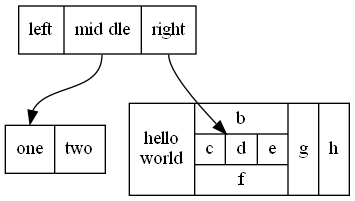
\includegraphics[width=\textwidth]{test_fig_1.png}
    \caption{My Current Pipeline for Terrain }
    \Description{My Current Pipeline for Terrain}
    \label{fig:teaser}
\end{teaserfigure}

\maketitle

\paragraph{Machine Learning:}

One promising and under-explored avenue is the application of machine learning
to terrain synthesis. Guerin et al. take this tack by training a conditional generative adversarial network
on a set of annotated DEM exemplars.

The most important virtue of machine learning approach lies in its versatility.
It can be used to fill in gaps from missing data, or to increase reslution using a kind of erision feature learnt from erosion simulations.

There is also a promising topic called
terrain amplification,
which could generate a high-resolution
terrain from a low-resolution input terrain with an image controlling its style.
This could be an important post-processing method in terrain generation procedures.

%%
%% The next two lines define the bibliography style to be used, and
%% the bibliography file.
\bibliographystyle{acmart/ACM-Reference-Format}

\end{document}
\endinput
